\documentclass[letterpaper,10pt,titlepage,fleqn]{article}

%example of setting the fleqn parameter to the article class -- the below sets the offset from flush left (fl)
\setlength{\mathindent}{1cm}

\usepackage{graphicx}                                        

\usepackage{amssymb}                                         
\usepackage{amsmath}                                         
\usepackage{amsthm}                                          
\usepackage{nopageno}
\usepackage{alltt}                                           
\usepackage{float}
\usepackage{color}
\usepackage{wasysym}
\usepackage{url}

\usepackage{balance}
\usepackage[TABBOTCAP, tight]{subfigure}
\usepackage{enumitem}

\usepackage{pstricks, pst-node}

%the following sets the geometry of the page
\usepackage{geometry}
\geometry{textheight=9in, textwidth=6.5in}

% random comment

\newcommand{\cred}[1]{{\color{red}#1}}
\newcommand{\cblue}[1]{{\color{blue}#1}}

\usepackage{hyperref}

\usepackage{textcomp}
\usepackage{listings}

\def\name{Sam Quinn}

%% The following metadata will show up in the PDF properties
\hypersetup{
  colorlinks = true,
  urlcolor = black,
  pdfauthor = {\name},
  pdfkeywords = {cs311 ``operating systems'' files filesystem I/O},
  pdftitle = {CS 311 Project},
  pdfsubject = {CS 311 Project},
  pdfpagemode = UseNone
}

\parindent = 0.0 in
\parskip = 0.2 in

\begin{document}

%to remove page numbers, set the page style to empty

\section*{Surface Integral}
\addtocounter{section}{1}

\hrule

For a scalar function \textit{f} over a surface parameterized by \textit{u} and \textit{v}, the surface is given by

 \numberwithin{equation}{section}

\begin{eqnarray}
  \Phi &=& \int\limits_s \textit{f} \text{d}a\\
   &=& \int\limits_s(\textit{u},\textit{v}) \mid \bold{T_\textit{u}}\times\bold{T_\textit{v}}\mid \text{d} \textit{u} \text{d} \textit{v}
\end{eqnarray}.
where $\bold{T_\textit{u}}$ and $\bold{T_\textit{v}}$ are tangent vectors and is the cross product.
For a vector functions over a surface, the surface integral is given by 
\begin{eqnarray}
 \Phi &=& \int\limits_s \bold{f} \cdot \text{d} \bold{a}\\
 &=& \int\limits_s (\mathbf{F} \cdot \bold{\hat{n}}) \text{d} \textit{a}\\
 &=& \int\limits_s \textit{f}_{x} \text{d} \textit{y} \text{d} \textit{z} + \textit{f}_{y} \text{d} \textit{z} \text{d} \textit{x}+\textit{f}_{z} \text{d} \textit{x}\text{d} \textit{y}
\end{eqnarray}.
where $\mathbf{a}$ $\cdot$ $\mathbf{b}$ is a dot product and $\mathbf{\hat{n}}$ is a unit normal vector. If $z$ = $f(x,y)$, the d$\mathbf{a}$ is given explicitly by
\begin{eqnarray}
d\mathbf{a} = \pm(- \frac{\partial z}{\partial x}\hat{x}-\frac{\partial z}{\partial y}\hat{y}+\hat{z} )\text{d}x\text{d}y
\end{eqnarray}.
If the surface is \textit{surface parameterized} using $u$ and $v$, then
\begin{eqnarray}
\Phi=\int\limits_s \bold{F} \cdot (\mathbf{T}_{u}\times \mathbf{T}_{v})\text{d}u\text{d}v
\end{eqnarray}.
\section*{Maxwells's Equations}
\addtocounter{section}{1}
\addtocounter{equation}{-7}
 \numberwithin{equation}{section}
\hrule

\centerline{\includegraphics[width=0.5\textwidth]{maxwell.eps}}
\subsection*{Integral form}

\begin{eqnarray}
 \oiint\limits_{\partial{\Omega}} \mathbf{E} \cdot \text{d} \mathbf{S} &=& \frac{1}{\varepsilon}_{0}\iiint\limits_{\Omega} p \text{d}V\\
\oiint\limits_{\partial{\Omega}} \mathbf{B} \cdot \text{d} \mathbf{S} &=& 0\\
 \oint _{\partial{\Sigma}} \mathbf{E} \cdot \text{d} \ell &=& - \frac{d}{dt} \iint \limits_{\Sigma} \mathbf{B} \cdot \text{d} \mathbf{S}\\
 \oint _{\partial{\Sigma}} \mathbf{B} \cdot \text{d} \ell &=& \mu_{0} \iint \limits_{\Sigma} (\mathbf{J}+\varepsilon_{0} \frac{\partial \mathbf{E}}{\partial t}) \cdot \text{d} \mathbf{S}
\end{eqnarray}.
\subsection*{Differential form}
\begin{eqnarray}
\nabla \cdot \mathbf{E} &=& \frac{p}{\varepsilon_{0}}\\
\nabla \cdot \mathbf{B} &=& 0\\
\nabla \times \mathbf{E} &=& -\frac{\partial{\mathbf{B}}}{\partial t}\\
\nabla \times \mathbf{B} &=& \mu_{0}(\mathbf{J}+\varepsilon_{0} \frac{\partial{\mathbf{E}}}{\partial t})
\end{eqnarray}.
\section*{Grading Policies}
\hrule

\begin{enumerate}
\item All project must be submitted electronically by 23:59:59 on the due date via TEACH – use "Check time on server" if unsure about your clock. TEACH time takes priority over your local computer.
\item Only a single late homework assignment allowed. Only allowed up to 7 calendar days late.
\item Submit late homework to your assigned TA via email.
\item Blatant disrespect to or by the TAs will not be tolerated. 
\item If you do not demo your project, you do not receive credit for it. 
\item When you make an appointment to demo, show up. Failure to show up will result in a grade penalty. Repeated offenses will result in no credit for the assignment. 
\item If your project does not compile, for any reason, no credit will be given.
\item Compilation will be on os-class. This server is the final say on whether your code compiles. 
\item No directories in you submissions. You will be penalized for including any sort of hierarchy.
\item All assignments submitted to TEACH. No late submissions will be accepted via TEACH.
\item Naming convention: CS311\_proj\textlangle x\textrangle \_\textlangle engr\_username\textrangle.tar.bz2. Fill \textlangle \textrangle  in with appropriate values.
\item No zip files will be accepted. You must use bzipped tar files.
\item All non-code documents must be created with LaTeX, by hand. This will be discussed in class.
\item All work must be done individually unless specifically allowed to work in groups.
\end{enumerate}

\section*{Learning Objectives}
\hrule

\begin{itemize}
\item Explain why multiprogramming is important for modern operating systems.
\item Explain the general structure of a multiprogrammed operating system.
\item Explain the purpose and operation of system calls.
\item Write a program utilizing system calls.
\item Write a program using a scripting language.
\item Write a program that uses regular expressions to parse input data.
\item Write a program that spawns processes and provides mutual exclusion for variables or other resources shared by the processes.
\item Write a program that uses sockets to implement a client/server system.
\item Explain how a common file system works, including structure, I/O operations, and security.
\item Describe the memory organization of a typical process in a common operating system.
\end{itemize}

\end{document}
